\section{Transiciones}

Las \textbf{transiciones} nos permiten pasar de un valor de propiedad a otro dada una duración. La sintaxis básica es la siguiente:
\begin{center}
    \textit{transition: propiedad duración}
\end{center}

Donde:
\begin{itemize}
    \item \textbf{propiedad}: especifica la propiedad que tendrá la transición.
    \item \textbf{duración}: especifica el tiempo de duración de la transición.
\end{itemize}

La propiedad \textit{transition} de CSS se le debe asignar al elemento que se desea que tenga una animación, pero de momento todavía no hace nada; en caso de que se omita alguno de los dos valores básicos anteriores, la animación no funcionará. Para hacer que la animación se haga, se debe establecer un nuevo valor para el valor \textit{propiedad} de \textit{transition}, esto debe ser fuera del elemento a animar, como por ejemplo, si hacemos que el puntero del mouse se ponga encima del elemento, cambie de tamaño:
\begin{lstlisting}
    div {
        /* Valor inicial de la propiedad a animar. */
        width: 100px;
        height: 100px;
        background: red;
        /* Establece la propiedad a animar y la duración. */
        transition: width 2s;
    }
    div:hover {
        /* Valor final de la propiedad a animar. */
        width: 300px;
    }
\end{lstlisting}

Como vemos en el ejemplo anterior, el elemento tiene un valor inicial, mientras que el mismo, pero con un evento distinto, tiene su valor final, esta estructura conforma la animación del elemento. En este caso, cuando se quite el puntero del mouse de encima del elemento, este volverá a su estado inicial.

En caso de animar varias propiedades de un elemento, simplemente se separan por comas:
\begin{lstlisting}
    div {
        /* Valor inicial de las propiedades a animar. */
        width: 100px;
        height: 100px;
        background: red;
        /* Establece las propiedades a animar y la duración. */
        transition: width 2s, height 2s;
    }
    div:hover {
        /* Valor final de las propiedades a animar. */
        width: 300px;
        height: 300px;
    }
\end{lstlisting}


\subsection{Velocidad de la transición}

La propiedad \textbf{transition-timming-function} de CSS permite cambiar la velocidad en la que la transición se crea dentro de la duración establecida, es decir, una animación puede durar cinco segundos en concretarse, pero esta puede comenzar lento, luego rápido y finalizar lento nuevamente, vemos los valores de esta propiedad:
\begin{itemize}
    \item \textbf{ease}: la transición comienza lento, luego rápido y termina lento (valor predeterminado).
    \item \textbf{linear}: la transición tiene la misma rapidez de comienzo a fin.
    \item \textbf{ease-in}: la transición tiene un comienzo lento.
    \item \textbf{ease-out}: la transición tiene un final lento.
    \item \textbf{ease-in-out}: la transición tiene un comienzo y final lento.
    \item \textbf{cubic-bezier(\textit{n},\textit{n},\textit{n},\textit{n})}: define tus propios valores para una función cúbica bezier (valores aceptados en cada parámetro: 0 y 1).
    \item \textbf{step-start}: la transición avanza según una cantidad \textit{n} de pasos, en este caso, solamente tiene un paso y comienza del lado izquierdo del elemento.
    \item \textbf{step-end}: la transición avanza según una cantidad \textit{n} de pasos, en este caso, solamente tiene un paso y comienza del lado derecho del elemento.
    \item \textbf{steps(\textit{n}, \textit{término})}: define tus propios valores para una función de \textit{steps} con \textit{n} cantidad de pasos y un término en el que se darán los pasos.
    \item \textbf{inherit}, \textbf{initial} y \textit{unset}.
\end{itemize}


\subsection{Retraso de la transición}

La propiedad \textbf{transition-delay} de CSS agrega un tiempo de retraso a la transición antes de que comience:
\begin{center}
    \textit{transition-delay: 2s;}
\end{center}

Entonces, la propiedad \textit{transition} puede ser especificada como:
\begin{lstlisting}
    div {
        transition-property: width;
        transition-duration: 2s;
        transition-timming-function: linear;
        transition-delay: 1s;
    }
\end{lstlisting}

O con su acceso directo:
\begin{center}
    \textit{transition: width 2s linear 1s;}
\end{center}



\section{Transformaciones}

Una \textbf{transformación} es un efecto que permite cambiar la forma, tamaño y posición de un elemento. CSS permite transformaciones 2D y 3D. Las transformaciones se consiguen mediante la propiedad \textbf{transform}.


\subsection{rotate()}

El método \textbf{rotate()} permite rotar un elemento x unidades de ángulos, recordemos las \textbf{Unidades de Ángulos}:
\begin{itemize}
    \item \textbf{deg}: grados, de 0 a 360 en un círculo.
    \item \textbf{grad}: gradianes, de 0 a 400 en un círculo.
    \item \textbf{rad}: radianes, hay 2$$\pi$$ (aproximadamente 6.28) en un círculo.
    \item \textbf{turn}: vueltas, hay 1 vuelta en un círculo. No es muy soportado por los buscadores.
\end{itemize}

Las figuras rotadas con valores positivos rotan en el sentido de las manecillas del reloj, si utiliza valores negativos, rotarán en sentido contrario. En la \textit{Figura \ref{fig: 52}} hay un ejemplo y su resultado:
\begin{lstlisting}
estilos.css
    /* Clase con rotación positiva. */
    .positive {
        width: 200px;
        height: 100px;
        margin-top: 30px;
        background-color: #32CD32;
        transform: rotate(10deg);
    }
    /* Clase con rotación negativa. */
    .negative {
        width: 200px;
        height: 100px;
        margin-top: 30px;
        background-color: #32CD32;
        transform: rotate(-10deg);
    }

prueba.html
    <div class="positive"></div>
    <br/>
    <div class="negative"></div>
\end{lstlisting}
\begin{figure}[H]
    \centering
    \caption{Método \textbf{rotate()} para rotar un elemento}
    \label{fig: 52}
    
\includegraphics[width=5cm]{ss/rotate.png}
\end{figure}


\subsection{transform-origin()}

El método \textbf{transform-origin()} permite cambiar la posición del eje del elemento transformado. Recordemos que cada elemento tiene un punto de origen el cual es el que se mueve entre transformaciones o animaciones, es como en vez de empujar o mover el elemento de sus contornos o márgenes, lo empujamos o movemos desde su eje, este eje es el centro del elemento por valor inicial. Este eje o punto de origen puede ser modificado mediante valores predeterminados, porcentaje o un largo, como vemos a continuación:
\begin{itemize}
    \item Valores aceptados para el eje X:
    \begin{itemize}
        \item \textbf{left}, \textbf{center}, \textbf{right} (izquierda, centro y derecha respectivamente), \textbf{porcentaje} (\%) y una Longitud (px, pt, cm, em, etc.).
        \item \textbf{initial} \textbf{inherit} y \textbf{unset}.
    \end{itemize}
    \item Valores aceptados para el eje y:
    \begin{itemize}
        \item \textbf{top}, \textbf{center}, \textbf{bottom} (parte superior, centro y parte inferior respectivamente), \textbf{porcentaje} (\%) y una Longitud (px, pt, cm, em, etc.).
        \item \textbf{initial}, \textbf{inherit} y \textbf{unset}.
    \end{itemize}
\end{itemize}

Se suele trabajar con porcentajes generalmente, pero puede combinar los valores predeterminados para conseguir la posición deseada, utilizaremos el ejemplo anterior para rotar dos elementos, pero cambiando el eje de ambos para que se aprecie cómo se ve la propiedad (\textit{Figura \ref{fig: 53}}):
\begin{lstlisting}
estilos.css
    /* Clase con rotación positiva con origen al 20 y 20 porciento. */
    .positive {
        width: 200px;
        height: 100px;
        margin-top: 30px;
        background-color: #32CD32;
        transform: rotate(10deg);
        transform-origin: 20% 20%;
    }
    /* Clase con rotación negativa con origen al 0 y 90 porciento. */
    .negative {
        width: 200px;
        height: 100px;
        margin-top: 30px;
        background-color: #32CD32;
        transform: rotate(-10deg);
        transform-origin: 0% 90%;
    }

prueba.html
    <div class="positive"></div>
    <br/>
    <div class="negative"></div>
\end{lstlisting}
\begin{figure}[H]
    \centering
    \caption{Función \textbf{transform-origin()} para cambiar el eje de un elemento}
    \label{fig: 53}
    
\includegraphics[width=5cm]{ss/transform-origin.png}
\end{figure}

Vemos entonces que los elementos cambian un poco su posición, esto es porque el eje modificado con \textit{transform-origin} está en otra ubicación.


\subsection{translate()}

El método \textbf{translate()} permite mover un elemento a una nueva posición según los valores dados para el eje X y eje Y. Valores positivos empujarán el elemento hacía abajo y hacía la derecha, mientras que los valores negativos hacía arriba y hacía la izquierda. El ejemplo en la \textit{Figura \ref{fig: 54}} muestra un elemento en su posición por defecto y la misma, pero trasladada unos píxeles:
\begin{lstlisting}
estilos.css
    /* Clase para contenedor original. */
    .default {
        width: 260px;
        height: 50px;
        margin-top: 30px;
        background-color: palegoldenrod;
        transform-origin: bottom center; 
    }
    /* Clase para contenedor movido 200px abajo y 100 a la derecha */
    .translated {
        width: 260px;
        height: 50px;
        background-color: palegoldenrod;
        transform-origin: bottom center;
        transform: translate(100px, 200px); 
    }

prueba.html
    <div class="default"></div>
    <div class="translated"></div>
\end{lstlisting}
\begin{figure}[H]
    \centering
    \caption{Método \textbf{translate()} para mover un elemento}
    \label{fig: 54}
    
\includegraphics[width=5cm]{ss/translate.png}
\end{figure}

Los elementos pueden ser movidos con las propiedades \textit{position}, \textit{top} y \textit{left} en conjunto y con los \textit{márgenes} del elemento, sin embargo, \textbf{translate} se utiliza en conjunto con las animaciones.


\subsection{skew()}

El método \textbf{skew()} (inclinar o inclinación) permite alterar la perspectiva de la figura en cuanto a su inclinación. Podemos hacer que la figura sea inclinada por medio de sus ejes x, y o por una cantidad de ángulos, como se ve en el ejemplo en la \textit{Figura \ref{fig: 55}}:
\begin{lstlisting}
estilos.css
    /* Clase para contenedor original. */
    .default {
        width: 100px;
        padding: 50px;
        background-color: #32CD32;
    }
    /* Clase para contenedor con inclinación de 30 grados. */
    .skewed_ang {
        position: fixed;
        left: 40px;
        width: 100px;
        padding: 50px;
        background-color: #32CD32;
        transform: skew(30deg);
    }
    /* Clase para contenedor con inclinación de 20 grados en el eje X
       y 50 grados en el eje Y. */
    .skewed_xy {
        position: fixed;
        top: 345px;
        left: 70px;
        width: 100px;
        padding: 50px;
        background-color: #32CD32;
        transform: skewX(20deg) skewY(50deg);
    }

prueba.html
    <div class="default"></div>
    <br/>
    <div class="skewed_ang"></div>
    <br/>
    <div class="skewed_xy"></div>
\end{lstlisting}
\begin{figure}[H]
    \centering
    \caption{Método \textbf{skew()} para inclinar un elemento}
    \label{fig: 55}
    
\includegraphics[width=5cm]{ss/skew.png}
\end{figure}

El método \textit{skew()} solamente recibe una cantidad de grados, mientras que \textbf{skewX()} y \textbf{skewY()} reciben también una sola cantidad de grados para el eje X, Y respectivamente, es así como se modifica la inclinación del elemento.


\subsection{scale()}

El método \textbf{scale()} permite incrementar o decrementar el tamaño de un elemento. Este método acepta dos parámetros, uno para el ancho y el otro para el alto, donde el valor 1 es el tamaño representa el tamaño original del elemento, 2 el doble y así sucesivamente, puede utilizar valores decimales, como se ve en la \textit{Figura \ref{fig: 56}}:
\begin{lstlisting}
estilos.css
    /* Clase para contenedor original. */
    .origin {
        width: 200px;
        height: 100px;
        background-color: #8BC34A;
        color:white;
    }
    /* Clase para contenedor con escala. */
    .first {
        width: 200px;
        height: 100px;
        background-color: #8BC34A;
        color:white;
        transform: scale(0.7, 0.7);
    }
    /* Clase para contenedor con escala. */
    .second {
        margin: 60px;
        width: 200px;
        height: 100px;
        background-color: #8bc34a;
        color:white;
        transform: scale(1.5,1.5);
    }

prueba.html
    <div class="origin">Hola mundo</div>
    <div class="first">Hola mundo</div>
    <div class="second">Hola mundo</div>
\end{lstlisting}
\begin{figure}[H]
    \centering
    \caption{Método \textbf{scale()} para cambiar escala de un elemento}
    \label{fig: 56}
    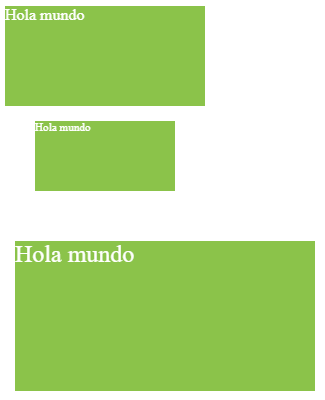
\includegraphics[width=5cm]{ss/scale.png}
\end{figure}

El ejemplo anterior utiliza el mismo valor tanto para el ancho como para el alto, pero se pueden utilizar distintos valores. En caso de que se omita el segundo parámetro, se tomará el valor del primero para el segundo.



\section{Animaciones}


\subsection{Keyframes \& animaciones}

La regla \textbf{keyframes} permite crear animaciones que pueden ser asignadas a un elemento mediante la propiedad \textbf{animation}. Estas animaciones tienen un inicio y un fin, el inicio puede ser la palabra reservada \textbf{from} o el 0\% y el final puede ser la palabra reservada \textbf{to} o el 100\% o se puede navegar a través de estos porcentajes para hacer una animación más detallada.

Puede animar todas las propiedades que desee las veces que sean. Las reglas \textit{keyframes} deben tener un nombre identificativo el cual será el que sea asignado a la propiedad \textit{animation}, como vemos en el siguiente ejemplo:
\begin{lstlisting}
    /* Animación con regla donde cambia el color de fondo. */
    @keyframes example {
        0%  {background-color: red;}
        50%  {background-color: yellow;}
        70%  {background-color: blue;}
        100% {background-color: green;}
    }
\end{lstlisting}

El nombre de la regla es \textit{example}, y cambia el color del fondo del elemento de rojo a amarillo, azul y verde, a través de los distintos porcentajes establecidos, esta animación entonces cambia gradualmente el color de fondo de un elemento.


\subsection{Propiedades de las animaciones}
\begin{itemize}
    \item \textbf{animation-name}: asigna una regla \textit{kewframes} a un elemento.
    \item \textbf{animation-duration}: establece la duración de la animación. Acepta valores en segundos. Si no se establece esta propiedad, la animación no comenzará, esto porque el valor por defecto es 0.
    \begin{lstlisting}
        div {
            animation-name: example;
            animation-duration: 3s;
        }
    \end{lstlisting}
    \item \textbf{animation-timming-function}: cambia la velocidad en la que la transición se crea dentro de la duración establecida. Los valores que acepta son los mismos que la propiedad \textit{transition-timming-function} en la sección \textbf{Transiciones} (\textbf{ease}, \textbf{linear}, \textbf{ease-in}, \textbf{ease-out}, \textbf{ease-in-out} y \textbf{cubic-bezier()}).
    \item \textbf{animation-delay}: agregar un retraso a la animación. Acepta valores en segundos o milisegundos.
    \begin{lstlisting}
        div {
            animation--timming-function: ease-in;
            animation-delay: 1s;
        }
    \end{lstlisting}
    \item \textbf{animation-iteration-count}: determina el número de veces que una animación se repetirá. Acepta valores enteros y la palabra reservada \textbf{infinite}, para repetir indefinidamente una animación. Si utiliza el valor 0, la animación nunca comenzará.
    \item \textbf{animation-direction}: indica el comportamiento de la regla o cómo esta es aplicada. Los valores que acepta son:
    \begin{itemize}
        \item \textit{normal}: la animación se aplica de 0\% a 100\%.
        \item \textit{reverse}: la animación se aplica de 100\% a 0\%.
        \item \textit{alternate}: la animación primero corre hacia adelante, luego hacia atrás, luego hacia adelante.
        \item \textit{alternate-reverse}: la animación primero corre hacia atrás, luego hacia adelante, luego hacia atrás.
    \end{itemize}
\end{itemize}

Dejamos un ejemplo para que lo pruebe y vea cómo se ve la animación:
\begin{lstlisting}
estilos.css
    /* Animación con regla donde el ancho pasa de 0px a 100px. */
    @keyframes colorchange {
        from { width: 0px; }
        to { width: 100px; }
    }
    /* Clase que define las propiedades de la animación con regla en contenedor. */
    .animation {
        animation-name: colorchange;
        animation-duration: 3s;
        animation-timing-function: ease-in;
        animation-delay: 1s;
        animation-iteration-count: infinite;
        animation-direction: reverse;
        height:100px;
        width:0px;
    }

prueba.html
    <div class="animation"></div>
\end{lstlisting}

Puede utilizar el \textbf{acceso directo} de la propiedad \textit{animation} de la siguiente forma:
\begin{center}
    \textit{animation: name duration timming-function delay iteration-count direction}
\end{center}
